\documentclass[14pt,aspectratio=169]{beamer}
\usefonttheme[onlymath]{serif}
\usepackage[normalem]{ulem}
\usepackage[T2A]{fontenc}
\usepackage[utf8]{inputenc}
\usepackage[english,russian]{babel}
\usepackage{amssymb,amsfonts,amsmath,mathtext}
\usepackage{cite,enumerate,float,indentfirst}
\usepackage{bm}
\usepackage{subfig}

\usepackage{lipsum}

\newcommand\blfootnote[1]{%
  \begingroup
  \renewcommand\thefootnote{}\footnote{#1}%
  \addtocounter{footnote}{-1}%
  \endgroup
}

\graphicspath{{images/}}

\usetheme{Pittsburgh}
\usecolortheme{whale}

\setbeamercolor{footline}{fg=blue}
\setbeamertemplate{footline}{
  \leavevmode%
  \hbox{%
  \begin{beamercolorbox}[wd=.333333\paperwidth,ht=2.25ex,dp=1ex,center]{}%
    Павлович В. В. | selatnick@gmail.com
  \end{beamercolorbox}%
  \begin{beamercolorbox}[wd=.333333\paperwidth,ht=2.25ex,dp=1ex,center]{}%
    Минск, 2017
  \end{beamercolorbox}%
  \begin{beamercolorbox}[wd=.333333\paperwidth,ht=2.25ex,dp=1ex,right]{}%
  Стр. \insertframenumber{} из \inserttotalframenumber \hspace*{2ex}
  \end{beamercolorbox}}%
  \vskip0pt%
}

\setbeamertemplate{footline}[frame number]{}
\setbeamertemplate{navigation symbols}{}
\setbeamertemplate{footline}{}

\newcommand{\itemi}{\item[\checkmark]}

\title{Domain adaptation}
\author{\small{Павлович Владислав}
\vspace{20pt}%
}
\date{\small{Минск, 2018}}

\begin{document}
\maketitle

\begin{frame}
\frametitle{Domain adaptation}
\begin{itemize}
\item Small [un]labeled dataset from target domain.
\item Huge labeled dataset in a relevant domain.
\end{itemize}
\end{frame}

\begin{frame}
\frametitle{Domain adaptation}
\center{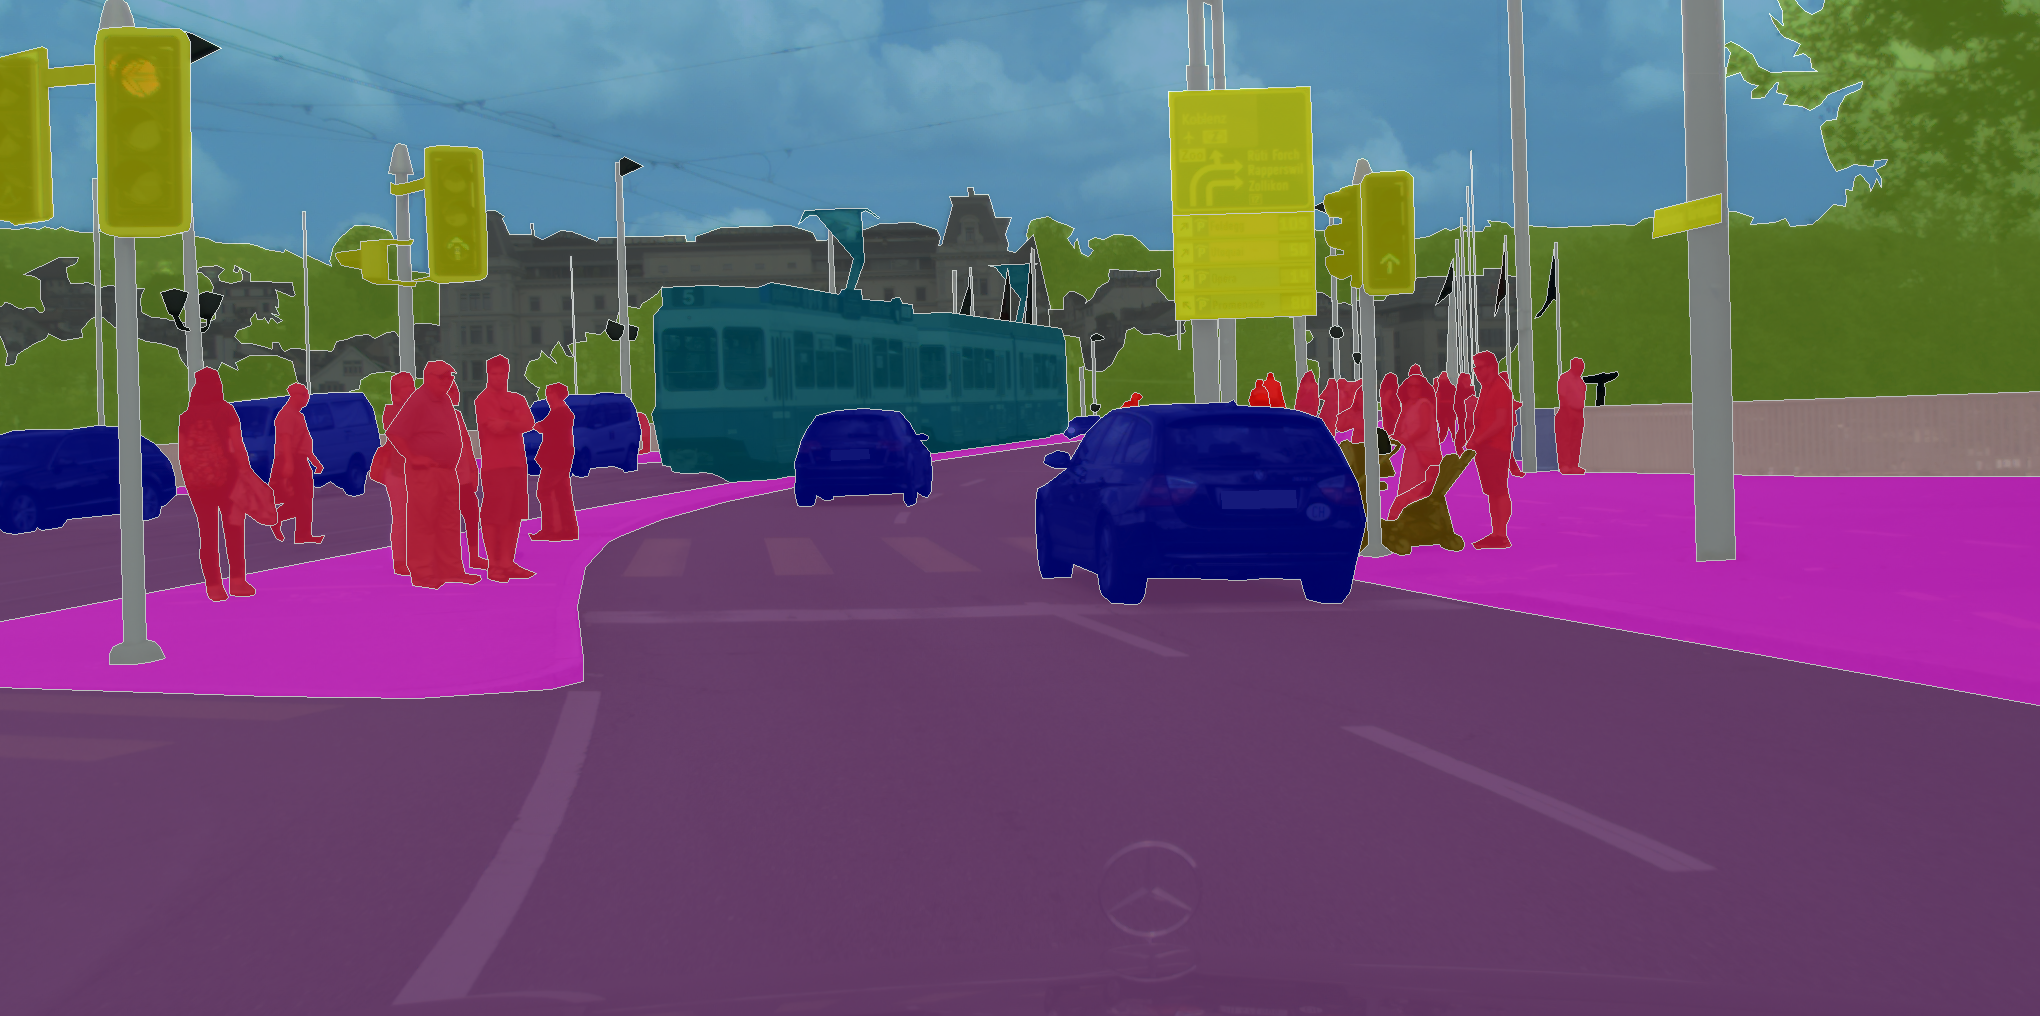
\includegraphics[width=0.9\linewidth]{segmentation_example.png}}
\end{frame}

\begin{frame}
\begin{figure}
\centering
\subfloat[GTA]{
  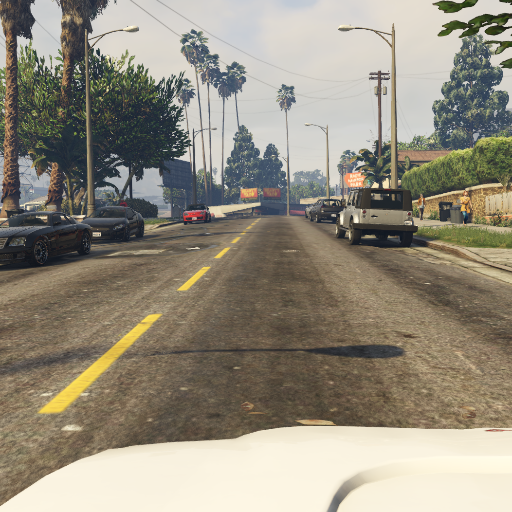
\includegraphics[width=0.4\linewidth]{domain_synthetic.png}
}
\subfloat[Cityscapes]{
  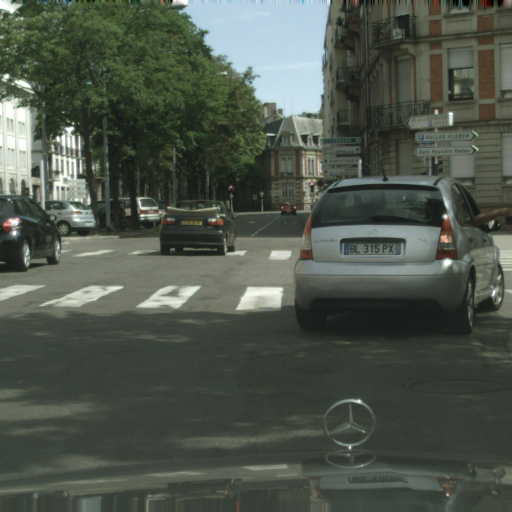
\includegraphics[width=0.4\linewidth]{domain_real.png}
}
\end{figure}
\end{frame}

\begin{frame}
\frametitle{Domain adaptation}
\begin{center}
  \begin{tabular}{|c|c|c|}\hline
    Model & Loss & Accuracy \\\hline
    GTA 64x64 & 0.5892 & 0.7049 \\\hline
    GTA 128x128 & 1.1422 & 0.6808 \\\hline
    GTA 256x256 & 1.0450 & 0.6714 \\\hline
    GTA 512x512 & 1.4202 & 0.6742 \\\hline
    Cityscapes 64x64 & 0.3859 & 0.8473 \\\hline
    Cityscapes 128x128 & 0.4728 & 0.7930 \\\hline
    Cityscapes 256x256 & 0.3717 & 0.8325 \\\hline
    Cityscapes 512x512 & 0.4498 & 0.8011 \\\hline
  \end{tabular}
\end{center}
\end{frame}

\begin{frame}
\frametitle{Notation}
\begin{itemize}
  \item Feature space $X$.
  \item Probability distribution $P(X)$.
  \item Domain $D = \left\{X, P(X)\right\}$.
  \item Objective prediction function $f(x) = P(Y|X)$.
\end{itemize}
\end{frame}

\begin{frame}
\frametitle{Notation}
\begin{itemize}
  \item $D^s = \left\{X, P_s(X)\right\}$.
  \item $D^t = \left\{X, P_t(X)\right\}$.
  \item $P_s(X) \to P_t(X)$.
\end{itemize}
\end{frame}

\begin{frame}
\frametitle{Domain adaptation}
\begin{itemize}
\item Shallow
\begin{itemize}
  \item Fine-tuning
\end{itemize}
\item Deep
\begin{itemize}
  \item SimGAN
  \item CyCADA
  \item GeoConGAN
\end{itemize}
\end{itemize}
\end{frame}

% \begin{frame}
% \frametitle{Notation}
% \begin{itemize}
%   \item We have 2 domains: $D^s, D^t$.
% \end{itemize}
% \end{frame}
%
% \begin{frame}
% \frametitle{TL classification}
% \begin{itemize}
%   \item Inductive.
%   \item Transductive.
%   \item Unsupervised.
% \end{itemize}
%
% DA is transductive!
% \begin{itemize}
%   \item $T^s = T^t$.
%   \item $D^s \neq D^t$.
% \end{itemize}
% Types of DA to domains:
% \begin{itemize}
%   \item Homogenous - $X^s = X^t$.
%   \item Heterogenous - $X^s \neq X^t$.
% \end{itemize}
% \end{frame}
%
% \begin{frame}
% \frametitle{Moar classification}
% \begin{itemize}
%   \item Supervised - small amount of labeled data in $D^t$.
%   \item Semi-supervised - small labeled and huge unlabled in $D^t$.
%   \item Unsupervised - only unlabled in $D^t$.
% \end{itemize}
% \end{frame}
%
% \begin{frame}
% \frametitle{General methods}
% \begin{itemize}
%   \item Discrepancy-based (fine-tuning).
%   \item Adversarial-based
%   \item Reconstruction-based.
% \end{itemize}
% \end{frame}

\begin{frame}
\frametitle{Fine-tuning methods}
\begin{itemize}
  \item Class criterion.
  \item Architecture criterion.
\end{itemize}
\end{frame}

\begin{frame}
\frametitle{Class criterion | Supervised}
\begin{itemize}
  \item Use pre-trained on ImageNet model as a universal feature extractor.
  and train a linear classifier (SVM) on extracted features.
  \item Fine-tune pre-trained model.
\end{itemize}
\end{frame}

\begin{frame}
\frametitle{Architecture criterion}
\center{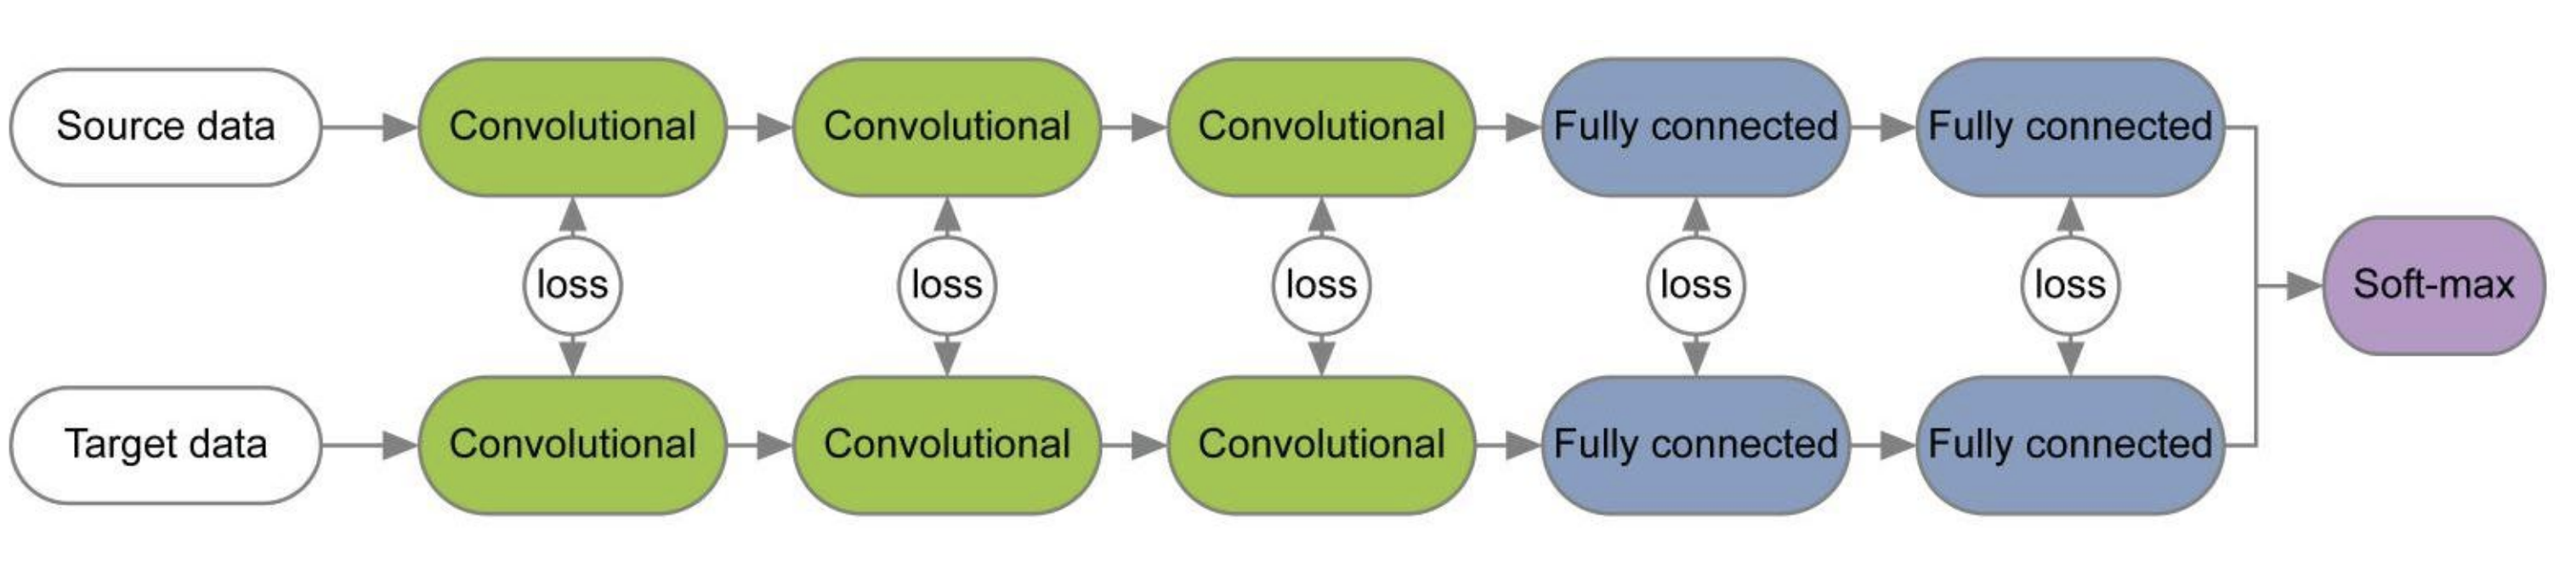
\includegraphics[width=0.9\linewidth]{architecture_criterion.png}}
\begin{align*}
  r_w(\theta_j^s; \theta_j^t) = \exp\left(||\theta_j^s - \theta_j^t||^2\right) - 1
\end{align*}
\end{frame}

\begin{frame}
\frametitle{SimGAN}
\center{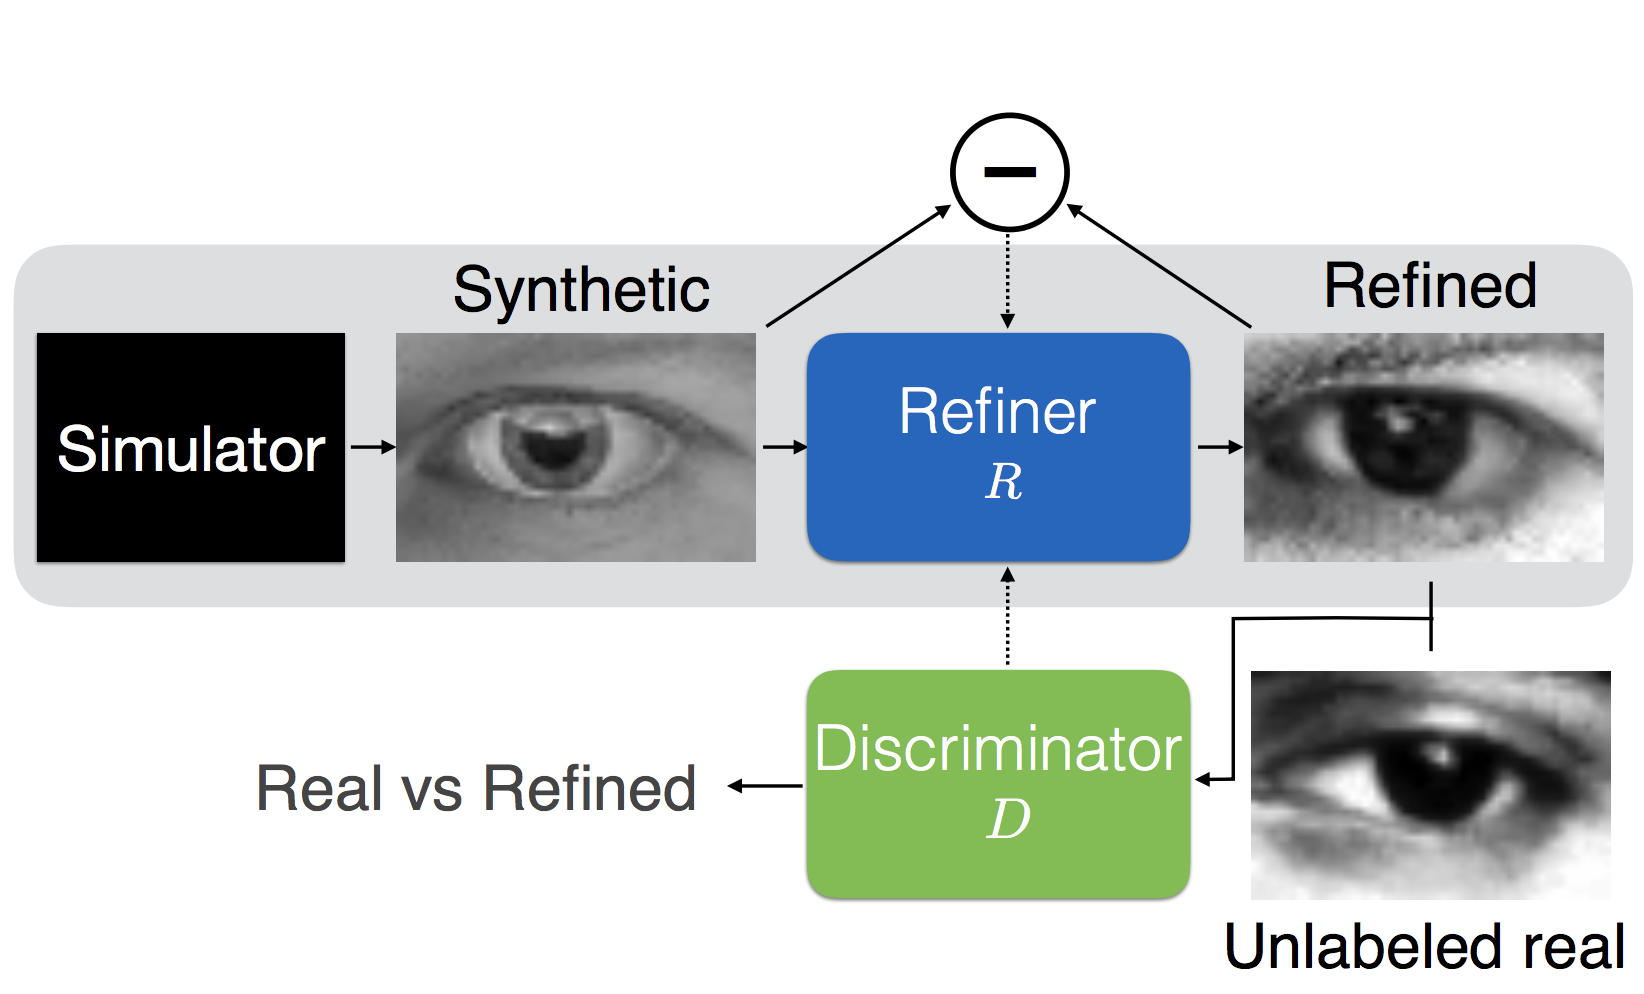
\includegraphics[width=0.7\linewidth]{simgan_overview.png}}
\blfootnote{Ashish S. et al. Learning from Simulated and Unsupervised Images through Adversarial
Training, 2016}
\end{frame}

\begin{frame}
\frametitle{SimGAN}
\begin{align*}
  L_R(\theta) &= \sum_i \ell_{real}(\theta; x_i, Y) + \lambda \ell_{reg}(\theta; x_i) = \\
  &= - \sum_i \log(1 - D_{\phi}(R_{\theta}(x_i))) + \\
  &+\lambda ||\psi(R_{\theta}(x_i)) - \psi(x_i)||
\end{align*}
$\psi$ - identity or any other transformation.
\blfootnote{Ashish S. et al. Learning from Simulated and Unsupervised Images through Adversarial
Training, 2016}
\end{frame}

\begin{frame}
\frametitle{SimGAN}
\center{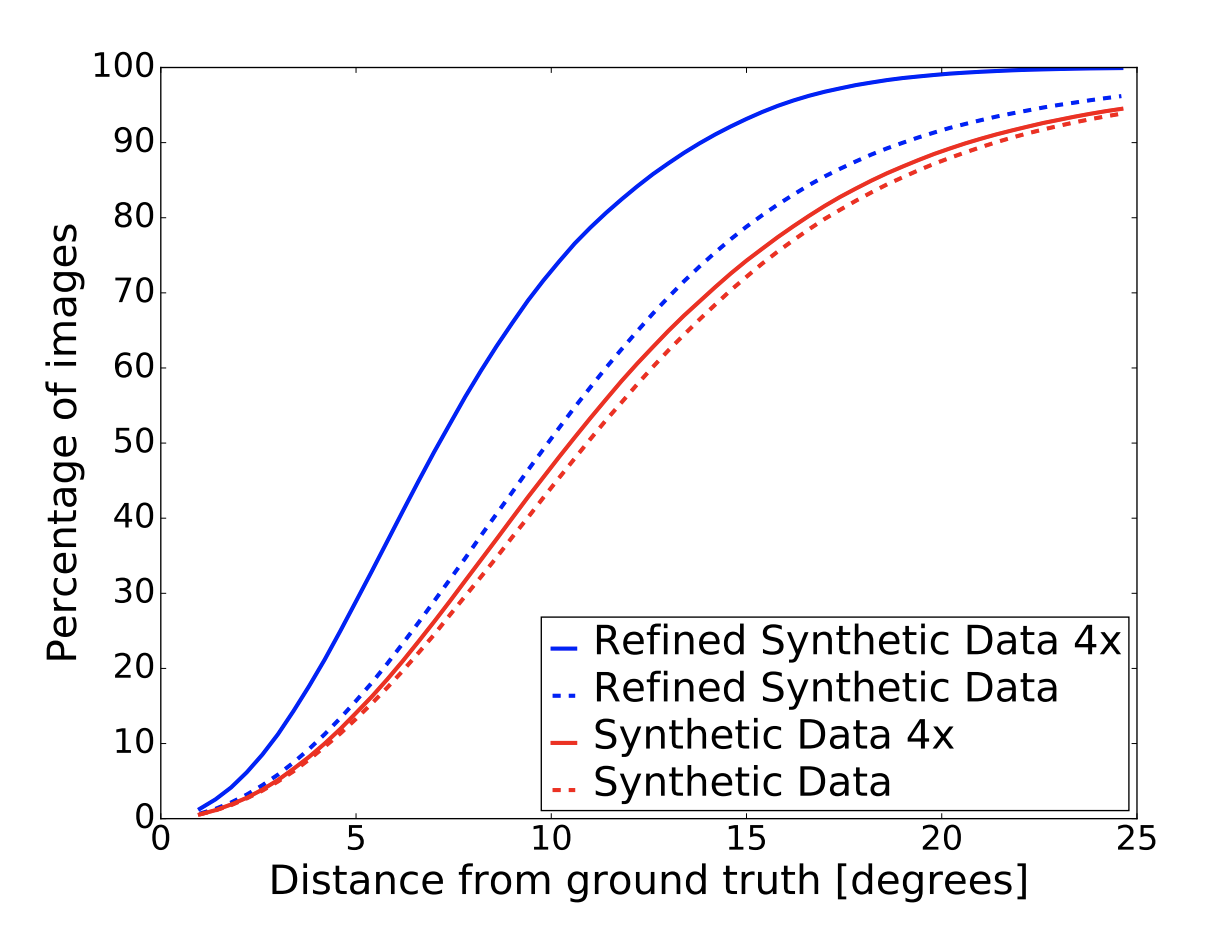
\includegraphics[width=0.5\linewidth]{simgan_plot.png}}
\blfootnote{Ashish S. et al. Learning from Simulated and Unsupervised Images through Adversarial
Training, 2016}
\end{frame}

\begin{frame}
\frametitle{SimGAN}
\center{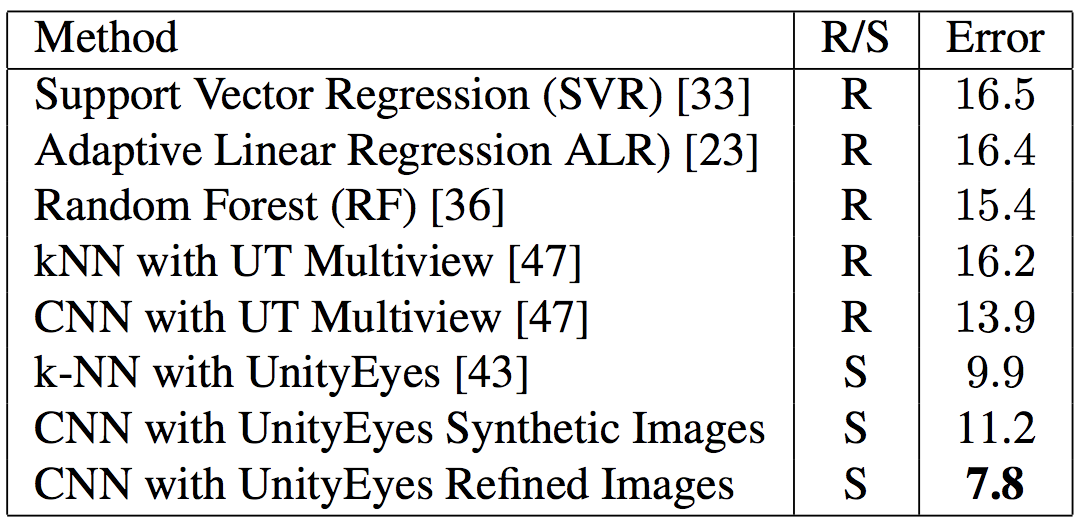
\includegraphics[width=0.8\linewidth]{simgan_results.png}}
\blfootnote{Ashish S. et al. Learning from Simulated and Unsupervised Images through Adversarial
Training, 2016}
\end{frame}

\begin{frame}
\frametitle{CycleGAN}
\center{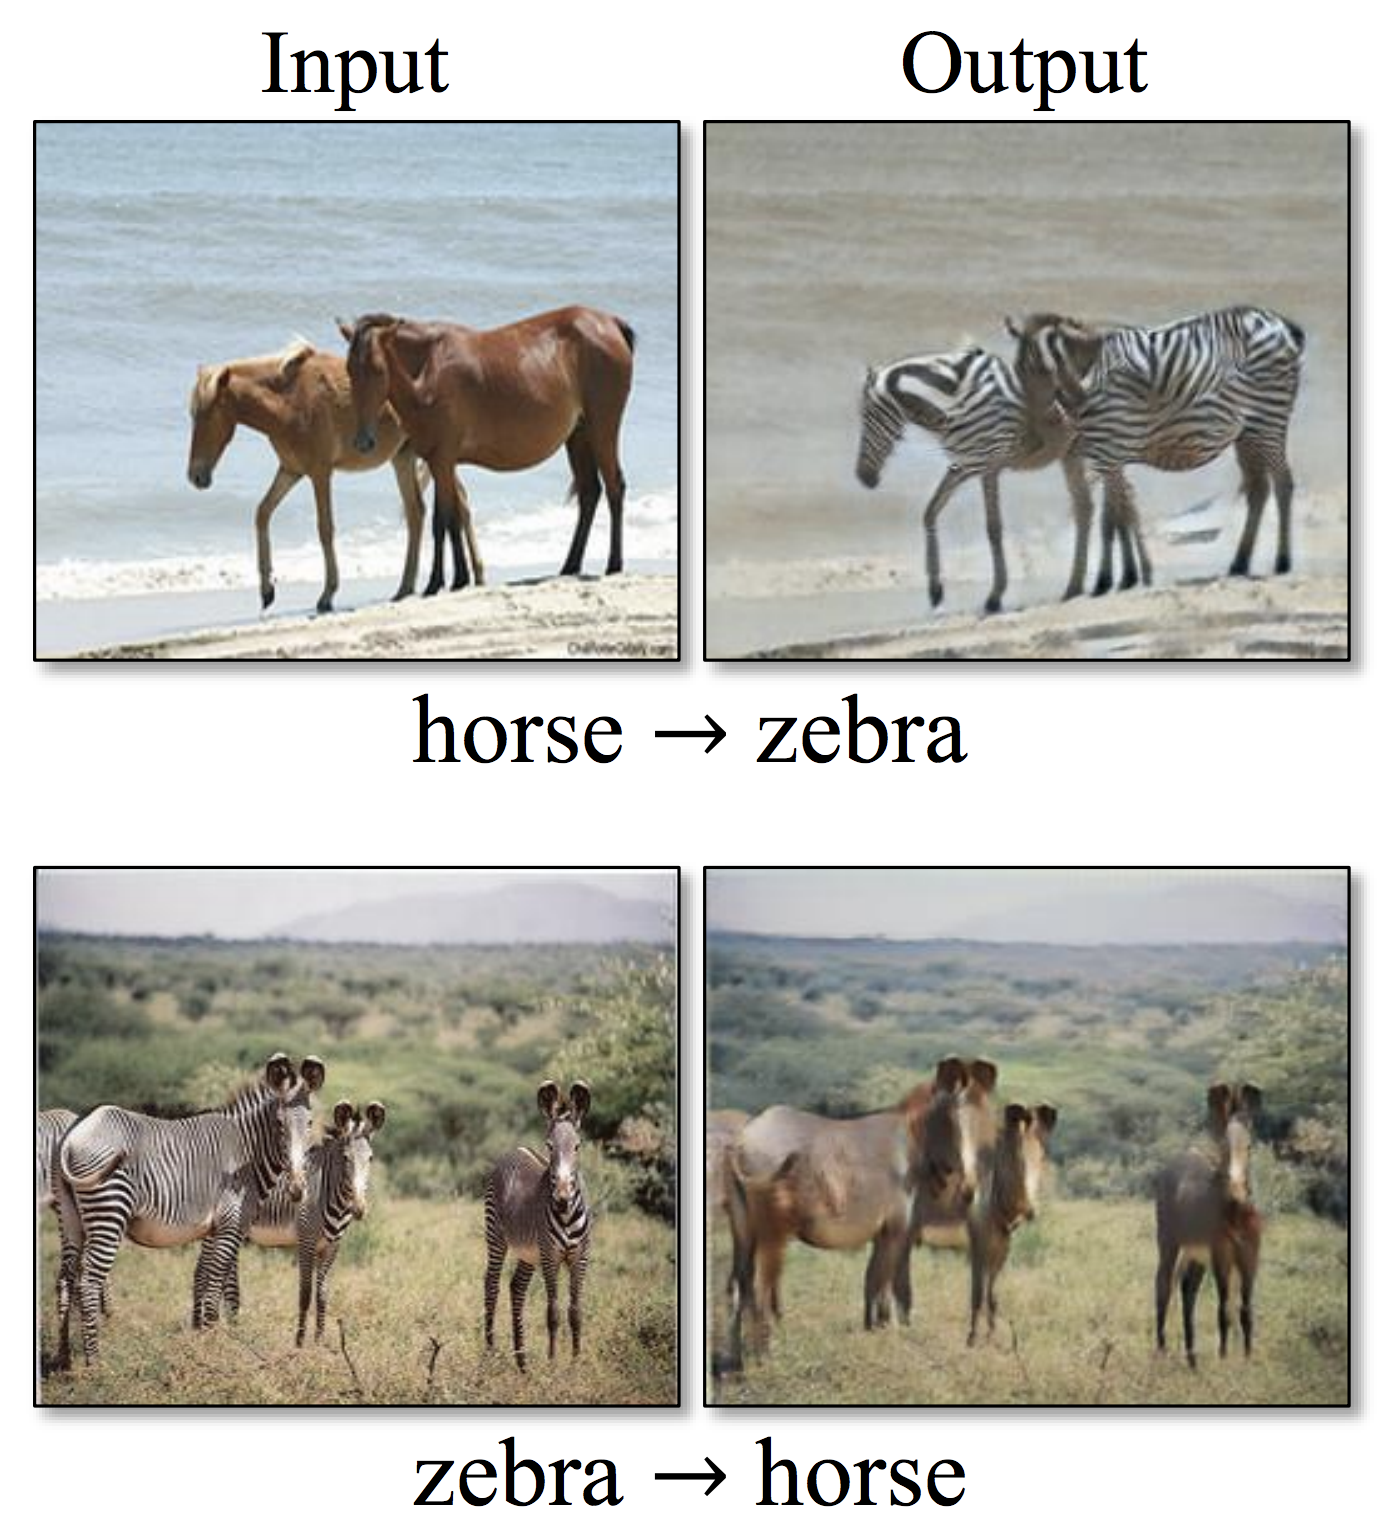
\includegraphics[height=0.3\linewidth]{cyclegan_samples.png}}
\blfootnote{Jun-Yan Zhu et al. Unpaired Image-to-Image Translation
using Cycle-Consistent Adversarial Networks, 2017}
\end{frame}

\begin{frame}
\frametitle{CycleGAN}
\center{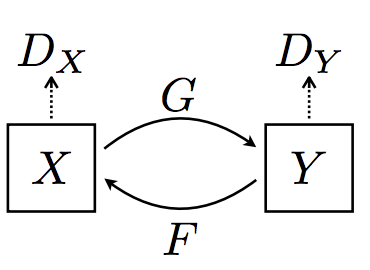
\includegraphics[height=0.3\linewidth]{cyclegan_scheme.png}}
\blfootnote{Jun-Yan Zhu et al. Unpaired Image-to-Image Translation
using Cycle-Consistent Adversarial Networks, 2017}
\end{frame}

\begin{frame}
\frametitle{CycleGAN}
\center{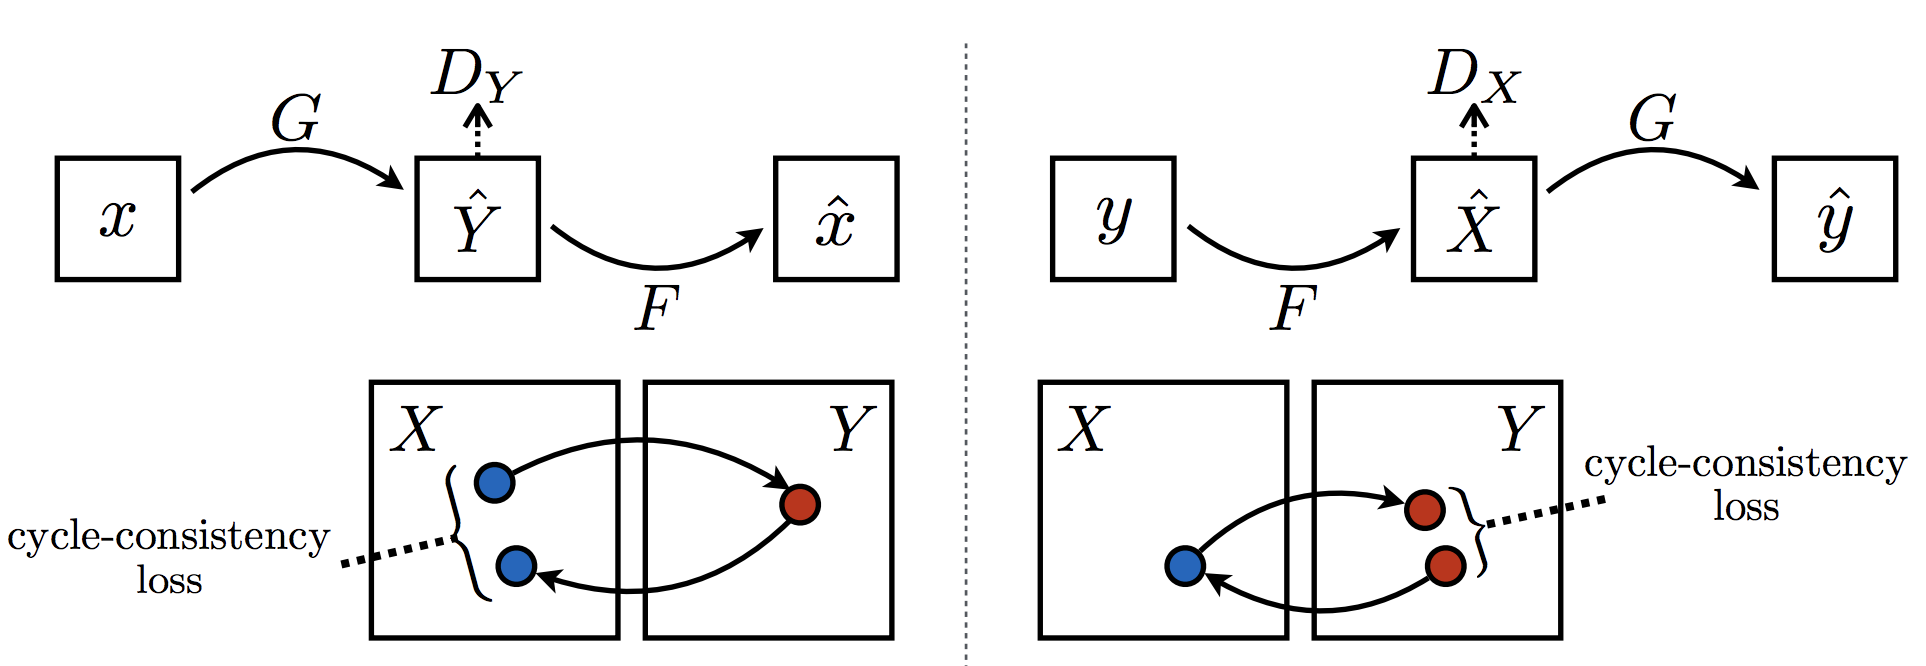
\includegraphics[height=0.3\linewidth]{cyclegan_loss.png}}
\blfootnote{Jun-Yan Zhu et al. Unpaired Image-to-Image Translation
using Cycle-Consistent Adversarial Networks, 2017}
\end{frame}

\begin{frame}
\frametitle{CycleGAN}
\begin{align*}
  L(G, F, D_X, D_Y) &= L_{GAN}(G, D_Y, X, Y) + \\
  & + L_{GAN}(F, D_X, Y, X) + \\
  & + \lambda L_{cyc}(G, F)\\
  L_{GAN}(G, D_Y, X, Y) & = E_{y \sim p_{data}(Y)}[\log D_Y(y)] +\\
  & + E_{x \sim p_{data}(X)}[\log(1 - D_Y(G(x))]\\
  L_{cyc}(G, F) & = E_{x \sim p_{data}(X)}[||F(G(x)) - x||_1] +\\
  & + E_{y \sim p_{data}(Y)}[||G(F(y)) - y||_1]\\
\end{align*}
\blfootnote{Jun-Yan Zhu et al. Unpaired Image-to-Image Translation
using Cycle-Consistent Adversarial Networks, 2017}
\end{frame}

\begin{frame}
\frametitle{CycleGAN}

\begin{figure}
\centering
\subfloat[Source]{
  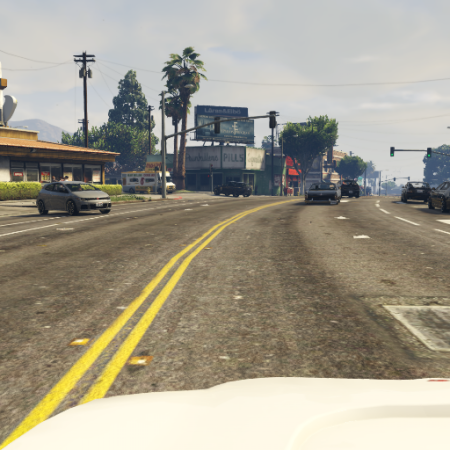
\includegraphics[width=0.4\linewidth]{gta_cyclegan_ex1.png}
}
\subfloat[Generated]{
  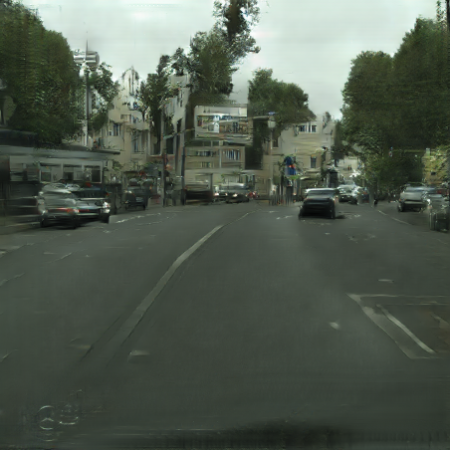
\includegraphics[width=0.4\linewidth]{gta_cyclegan_ex2.png}
}
\end{figure}
\end{frame}

\begin{frame}
\frametitle{CyCADA}
\center{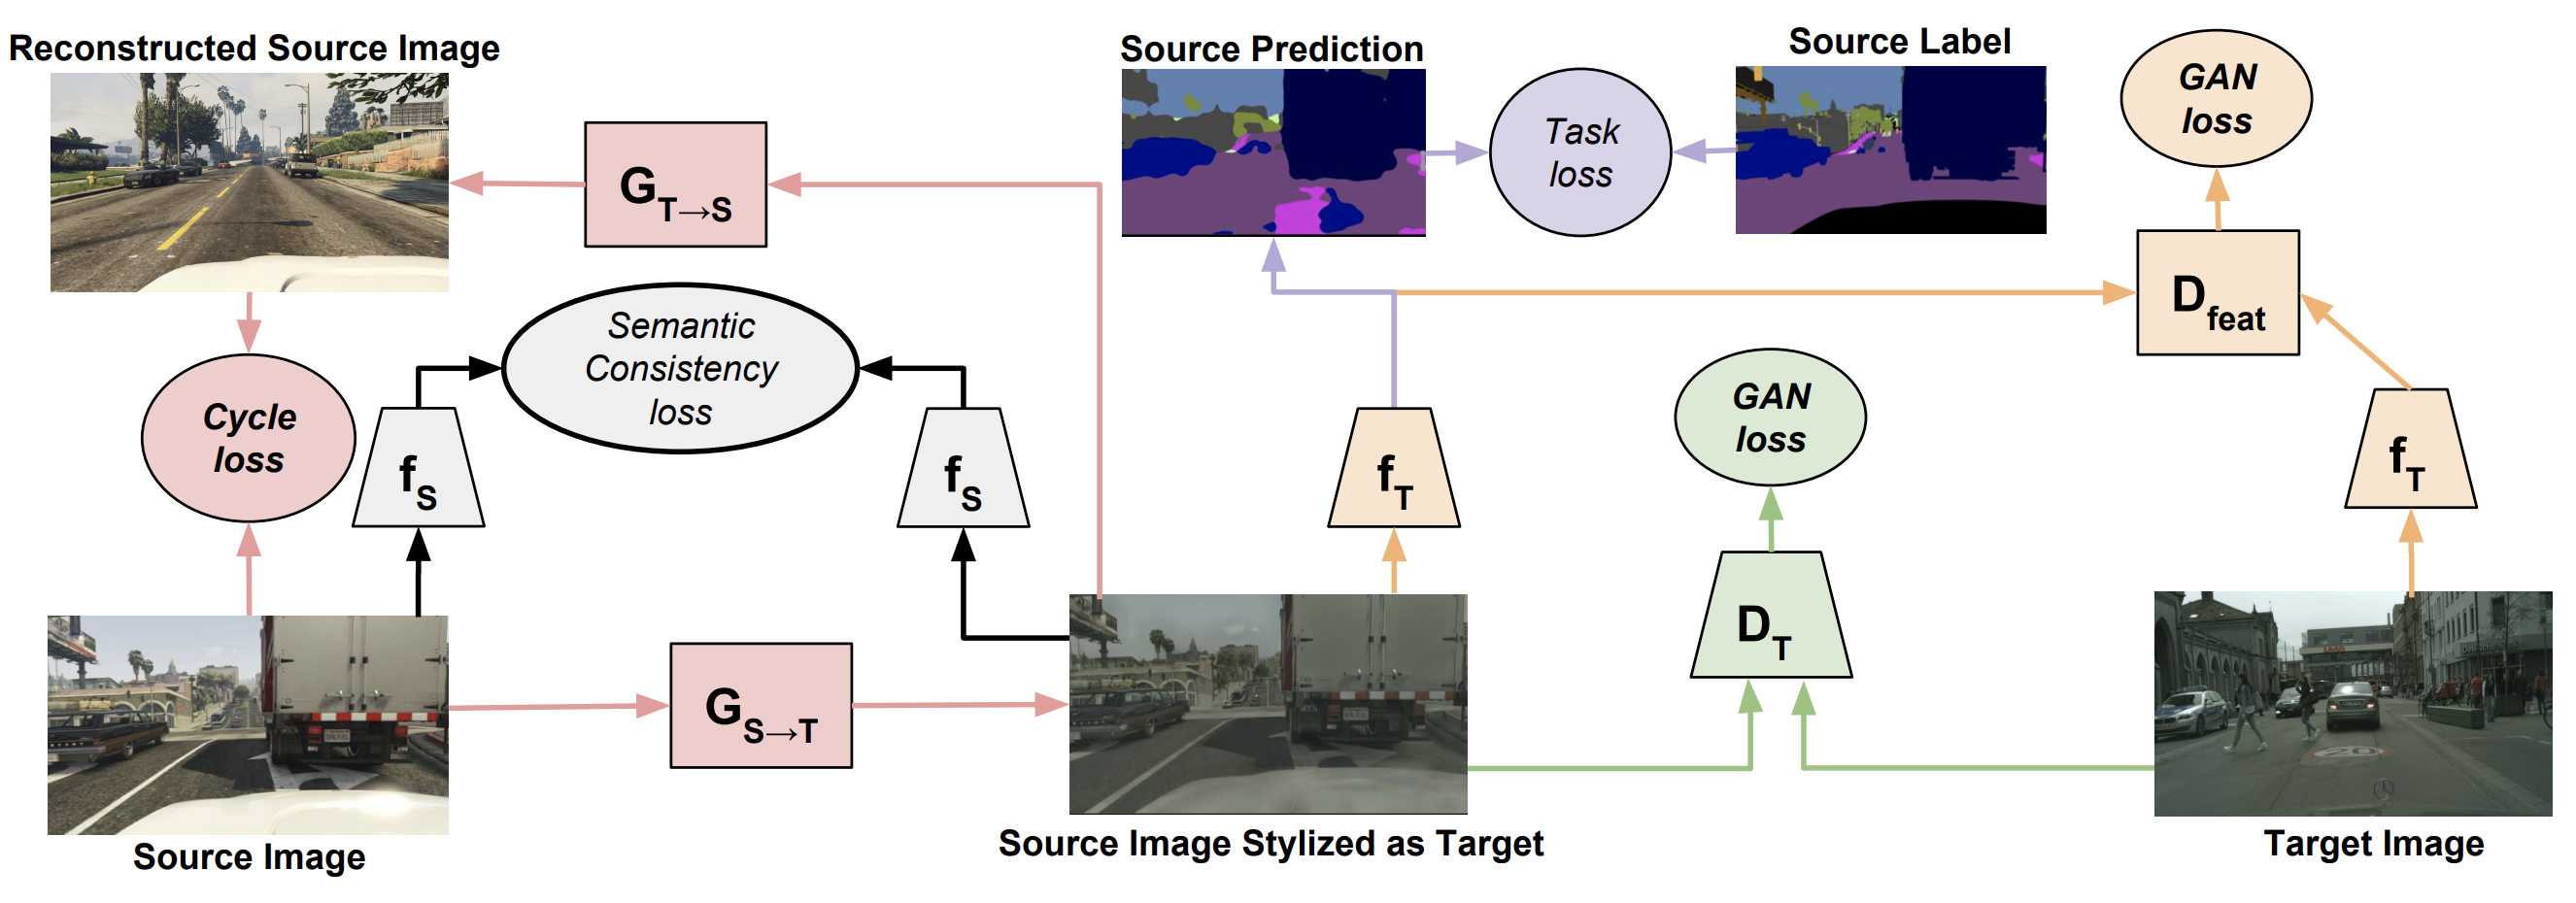
\includegraphics[width=1.0\linewidth]{cycada_scheme.png}}
\blfootnote{Judy Hoffman et al. CYCADA: cycle-consistent adversarial domain adaptation, 2017}
\end{frame}

\begin{frame}
\frametitle{CyCADA}
\center{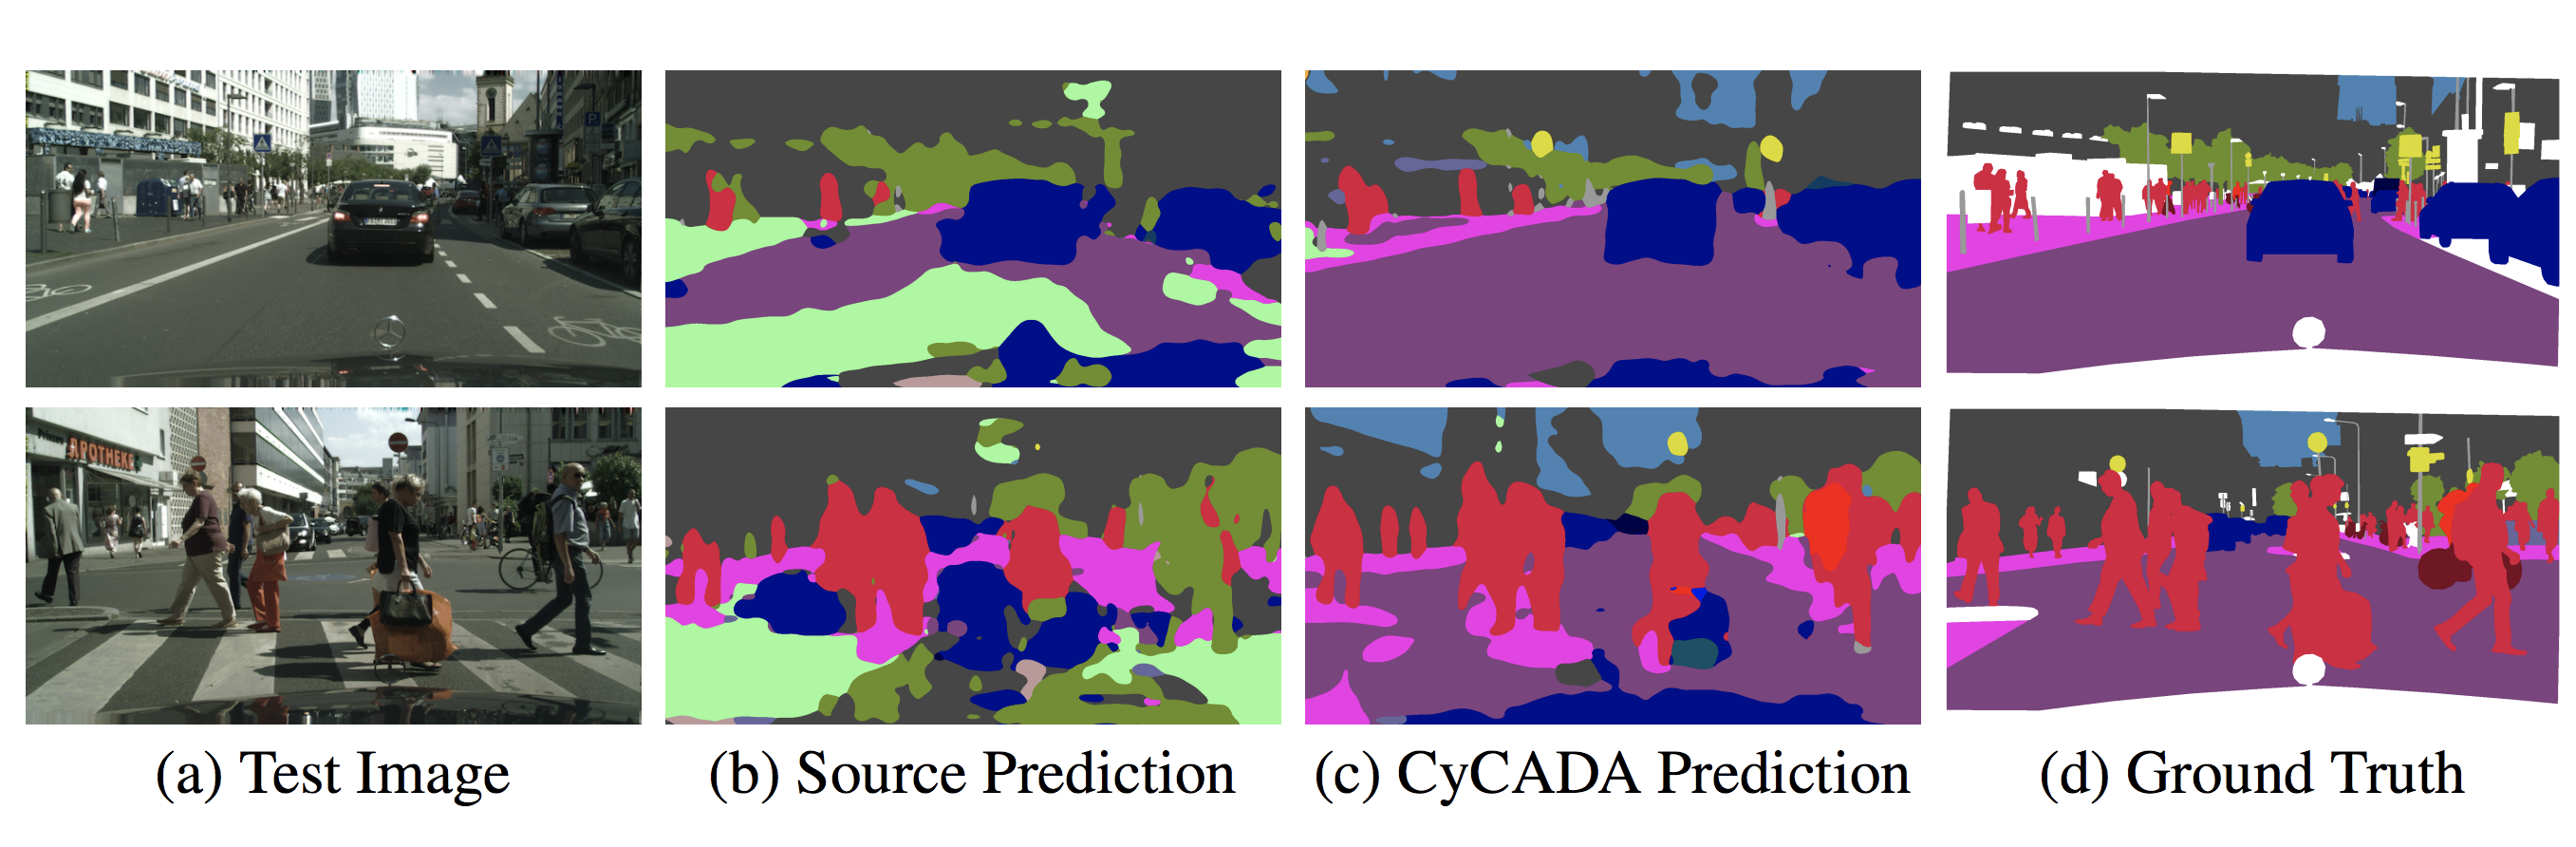
\includegraphics[width=1.0\linewidth]{cycada_example.png}}
\blfootnote{Judy Hoffman et al. CYCADA: cycle-consistent adversarial domain adaptation, 2017}
\end{frame}

\begin{frame}
\frametitle{CyCADA}
\begin{align*}
  &L_{task}(f_S, X_S, Y_S) = -E_{(x_s, y_s)\sim(X_S, Y_S)}\sum_{k = 1}^K\log(\sigma(f_S^{(k)}(x_s)))\\
\end{align*}
\begin{align*}
  L_{sem}(G_{S\to T}, G_{T\to S}, X_S, X_T, f_S) = & L_{task}(f_S, G_{T\to S}(X_T), p(f_S, X_T)) +\\
  & + L_{task}(f_S, G_{S\to T}(X_S), p(f_S, X_S))
\end{align*}
\blfootnote{Judy Hoffman et al. CYCADA: cycle-consistent adversarial domain adaptation, 2017}
\end{frame}

\begin{frame}
\frametitle{CyCADA}
\center{\begin{tabular}{|c|c|}\hline
Method & mIOU \\\hline
Source only & 21.7 \\\hline
CyCADA feat-only & 31.7 \\\hline
CyCADA pixel-only & 37 \\\hline
CyCADA pixel+feat & 39.5 \\\hline
\end{tabular}}
\end{frame}

\begin{frame}
\frametitle{GeoConGAN}
\center{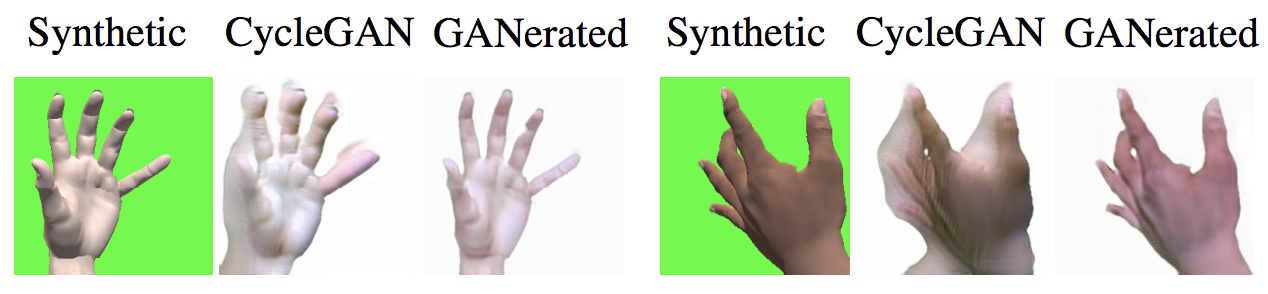
\includegraphics[width=1.0\linewidth]{geocongan_samples.png}}
\blfootnote{Franziska Mueller et al. GANerated Hands for Real-Time 3D Hand Tracking from Monocular RGB, 2018}
\end{frame}

\begin{frame}
\frametitle{GeoConGAN}
\begin{itemize}
  \item Based on CycleGAN.
  \item Extra cross-entropy loss for segmented images to preserve annotations.
\end{itemize}
\blfootnote{Franziska Mueller et al. GANerated Hands for Real-Time 3D Hand Tracking from Monocular RGB, 2018}
\end{frame}

\begin{frame}
\frametitle{GeoConGAN}
\center{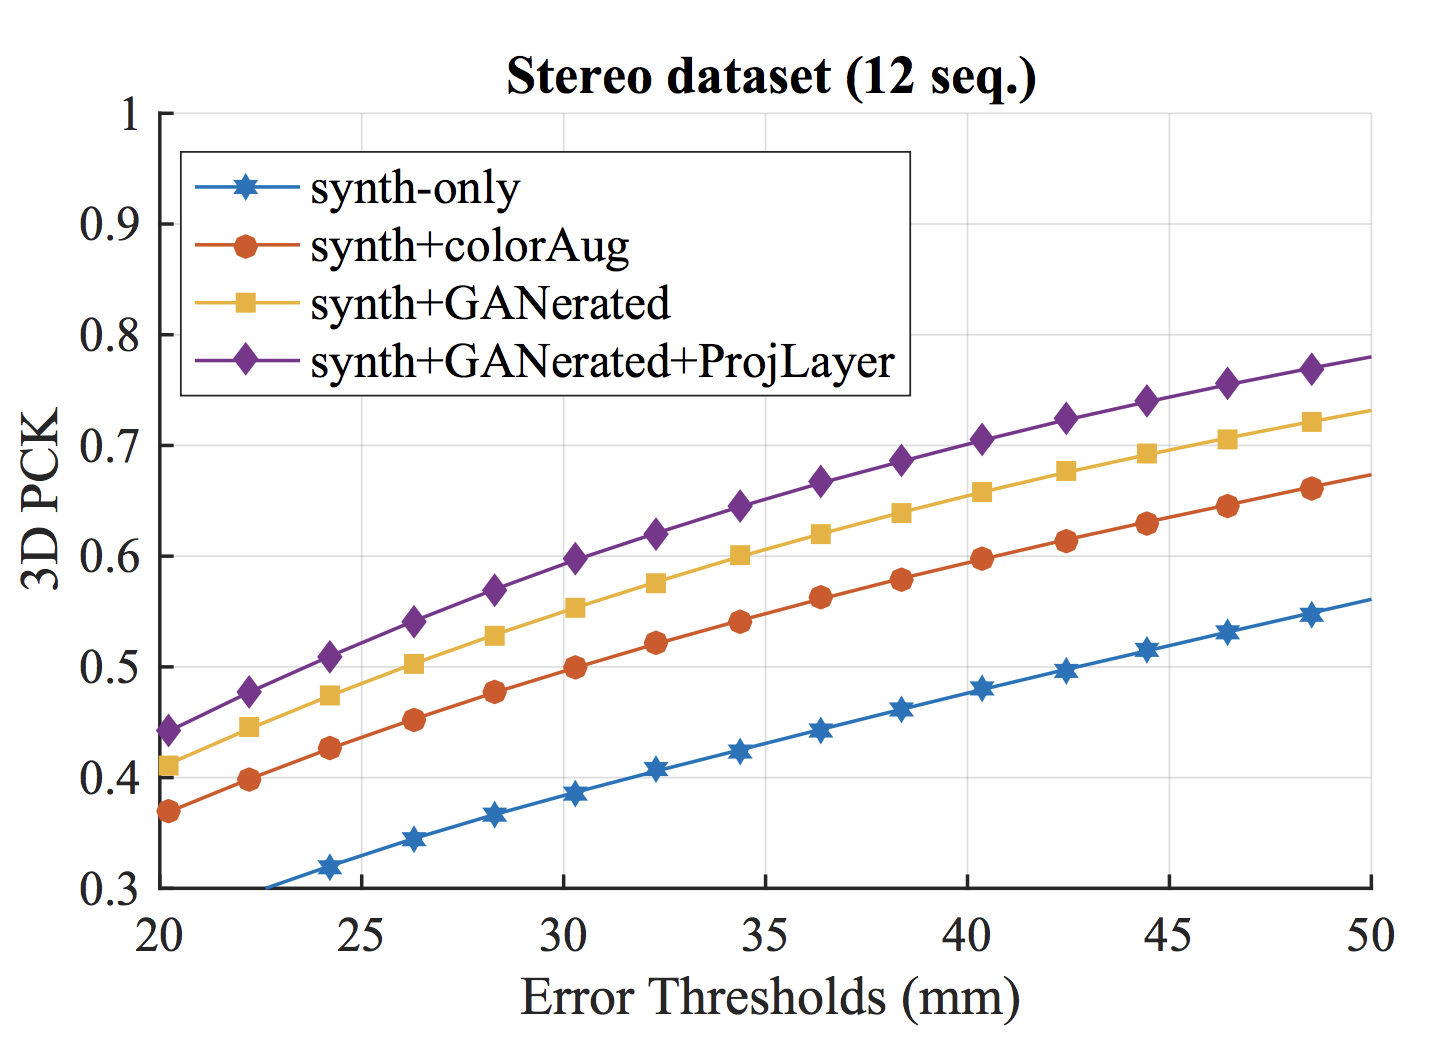
\includegraphics[height=0.4\linewidth]{geocongan_plot.png}}
\blfootnote{Franziska Mueller et al. GANerated Hands for Real-Time 3D Hand Tracking from Monocular RGB, 2018}
\end{frame}

\begin{frame}
\frametitle{Domain adaptation}
\center{Thank You!}
\end{frame}

\end{document}
